\documentclass[]{article}
\usepackage{lmodern}
\usepackage{amssymb,amsmath}
\usepackage{ifxetex,ifluatex}
\usepackage{fixltx2e} % provides \textsubscript
\ifnum 0\ifxetex 1\fi\ifluatex 1\fi=0 % if pdftex
  \usepackage[T1]{fontenc}
  \usepackage[utf8]{inputenc}
\else % if luatex or xelatex
  \ifxetex
    \usepackage{mathspec}
  \else
    \usepackage{fontspec}
  \fi
  \defaultfontfeatures{Ligatures=TeX,Scale=MatchLowercase}
\fi
% use upquote if available, for straight quotes in verbatim environments
\IfFileExists{upquote.sty}{\usepackage{upquote}}{}
% use microtype if available
\IfFileExists{microtype.sty}{%
\usepackage{microtype}
\UseMicrotypeSet[protrusion]{basicmath} % disable protrusion for tt fonts
}{}
\usepackage[margin=1in]{geometry}
\usepackage{hyperref}
\hypersetup{unicode=true,
            pdftitle={Class 05: Graphics and Plots with R},
            pdfauthor={Amy Prichard},
            pdfborder={0 0 0},
            breaklinks=true}
\urlstyle{same}  % don't use monospace font for urls
\usepackage{color}
\usepackage{fancyvrb}
\newcommand{\VerbBar}{|}
\newcommand{\VERB}{\Verb[commandchars=\\\{\}]}
\DefineVerbatimEnvironment{Highlighting}{Verbatim}{commandchars=\\\{\}}
% Add ',fontsize=\small' for more characters per line
\usepackage{framed}
\definecolor{shadecolor}{RGB}{248,248,248}
\newenvironment{Shaded}{\begin{snugshade}}{\end{snugshade}}
\newcommand{\KeywordTok}[1]{\textcolor[rgb]{0.13,0.29,0.53}{\textbf{#1}}}
\newcommand{\DataTypeTok}[1]{\textcolor[rgb]{0.13,0.29,0.53}{#1}}
\newcommand{\DecValTok}[1]{\textcolor[rgb]{0.00,0.00,0.81}{#1}}
\newcommand{\BaseNTok}[1]{\textcolor[rgb]{0.00,0.00,0.81}{#1}}
\newcommand{\FloatTok}[1]{\textcolor[rgb]{0.00,0.00,0.81}{#1}}
\newcommand{\ConstantTok}[1]{\textcolor[rgb]{0.00,0.00,0.00}{#1}}
\newcommand{\CharTok}[1]{\textcolor[rgb]{0.31,0.60,0.02}{#1}}
\newcommand{\SpecialCharTok}[1]{\textcolor[rgb]{0.00,0.00,0.00}{#1}}
\newcommand{\StringTok}[1]{\textcolor[rgb]{0.31,0.60,0.02}{#1}}
\newcommand{\VerbatimStringTok}[1]{\textcolor[rgb]{0.31,0.60,0.02}{#1}}
\newcommand{\SpecialStringTok}[1]{\textcolor[rgb]{0.31,0.60,0.02}{#1}}
\newcommand{\ImportTok}[1]{#1}
\newcommand{\CommentTok}[1]{\textcolor[rgb]{0.56,0.35,0.01}{\textit{#1}}}
\newcommand{\DocumentationTok}[1]{\textcolor[rgb]{0.56,0.35,0.01}{\textbf{\textit{#1}}}}
\newcommand{\AnnotationTok}[1]{\textcolor[rgb]{0.56,0.35,0.01}{\textbf{\textit{#1}}}}
\newcommand{\CommentVarTok}[1]{\textcolor[rgb]{0.56,0.35,0.01}{\textbf{\textit{#1}}}}
\newcommand{\OtherTok}[1]{\textcolor[rgb]{0.56,0.35,0.01}{#1}}
\newcommand{\FunctionTok}[1]{\textcolor[rgb]{0.00,0.00,0.00}{#1}}
\newcommand{\VariableTok}[1]{\textcolor[rgb]{0.00,0.00,0.00}{#1}}
\newcommand{\ControlFlowTok}[1]{\textcolor[rgb]{0.13,0.29,0.53}{\textbf{#1}}}
\newcommand{\OperatorTok}[1]{\textcolor[rgb]{0.81,0.36,0.00}{\textbf{#1}}}
\newcommand{\BuiltInTok}[1]{#1}
\newcommand{\ExtensionTok}[1]{#1}
\newcommand{\PreprocessorTok}[1]{\textcolor[rgb]{0.56,0.35,0.01}{\textit{#1}}}
\newcommand{\AttributeTok}[1]{\textcolor[rgb]{0.77,0.63,0.00}{#1}}
\newcommand{\RegionMarkerTok}[1]{#1}
\newcommand{\InformationTok}[1]{\textcolor[rgb]{0.56,0.35,0.01}{\textbf{\textit{#1}}}}
\newcommand{\WarningTok}[1]{\textcolor[rgb]{0.56,0.35,0.01}{\textbf{\textit{#1}}}}
\newcommand{\AlertTok}[1]{\textcolor[rgb]{0.94,0.16,0.16}{#1}}
\newcommand{\ErrorTok}[1]{\textcolor[rgb]{0.64,0.00,0.00}{\textbf{#1}}}
\newcommand{\NormalTok}[1]{#1}
\usepackage{graphicx,grffile}
\makeatletter
\def\maxwidth{\ifdim\Gin@nat@width>\linewidth\linewidth\else\Gin@nat@width\fi}
\def\maxheight{\ifdim\Gin@nat@height>\textheight\textheight\else\Gin@nat@height\fi}
\makeatother
% Scale images if necessary, so that they will not overflow the page
% margins by default, and it is still possible to overwrite the defaults
% using explicit options in \includegraphics[width, height, ...]{}
\setkeys{Gin}{width=\maxwidth,height=\maxheight,keepaspectratio}
\IfFileExists{parskip.sty}{%
\usepackage{parskip}
}{% else
\setlength{\parindent}{0pt}
\setlength{\parskip}{6pt plus 2pt minus 1pt}
}
\setlength{\emergencystretch}{3em}  % prevent overfull lines
\providecommand{\tightlist}{%
  \setlength{\itemsep}{0pt}\setlength{\parskip}{0pt}}
\setcounter{secnumdepth}{0}
% Redefines (sub)paragraphs to behave more like sections
\ifx\paragraph\undefined\else
\let\oldparagraph\paragraph
\renewcommand{\paragraph}[1]{\oldparagraph{#1}\mbox{}}
\fi
\ifx\subparagraph\undefined\else
\let\oldsubparagraph\subparagraph
\renewcommand{\subparagraph}[1]{\oldsubparagraph{#1}\mbox{}}
\fi

%%% Use protect on footnotes to avoid problems with footnotes in titles
\let\rmarkdownfootnote\footnote%
\def\footnote{\protect\rmarkdownfootnote}

%%% Change title format to be more compact
\usepackage{titling}

% Create subtitle command for use in maketitle
\newcommand{\subtitle}[1]{
  \posttitle{
    \begin{center}\large#1\end{center}
    }
}

\setlength{\droptitle}{-2em}

  \title{Class 05: Graphics and Plots with R}
    \pretitle{\vspace{\droptitle}\centering\huge}
  \posttitle{\par}
    \author{Amy Prichard}
    \preauthor{\centering\large\emph}
  \postauthor{\par}
      \predate{\centering\large\emph}
  \postdate{\par}
    \date{January 25th, 2019}


\begin{document}
\maketitle

\subsection{\texorpdfstring{This is some narrative text that I can style
\textbf{bold} and \emph{italic} and add links to
\href{https://rmarkdown.rstudio.com/articles_report_from_r_script.html}{webpages}}{This is some narrative text that I can style bold and italic and add links to webpages}}\label{this-is-some-narrative-text-that-i-can-style-bold-and-italic-and-add-links-to-webpages}

\textbf{Section 2A}: \emph{LINE PLOT}

\begin{Shaded}
\begin{Highlighting}[]
\NormalTok{weight<-}\KeywordTok{read.table}\NormalTok{(}\StringTok{"bimm143_05_rstats/weight_chart.txt"}\NormalTok{, }\DataTypeTok{header=}\OtherTok{TRUE}\NormalTok{)}
        \CommentTok{# header=TRUE reads in the first lines as column names}
\KeywordTok{plot}\NormalTok{(weight, }\DataTypeTok{pch=}\DecValTok{15}\NormalTok{, }\DataTypeTok{cex=}\FloatTok{1.5}\NormalTok{, }\DataTypeTok{lwd=}\DecValTok{2}\NormalTok{, }\DataTypeTok{ylim=}\KeywordTok{c}\NormalTok{(}\DecValTok{2}\NormalTok{,}\DecValTok{10}\NormalTok{), }\DataTypeTok{xlab=}\StringTok{"Age (months)"}\NormalTok{, }\DataTypeTok{ylab=}\StringTok{"Weight (kg)"}\NormalTok{, }\DataTypeTok{main=}\StringTok{"Baby Weight vs. Age"}\NormalTok{, }\DataTypeTok{type=}\StringTok{"o"}\NormalTok{)}
\end{Highlighting}
\end{Shaded}


\includegraphics{class05_files/figure-latex/unnamed-chunk-1-1.pdf}

\textbf{Section 2B}: \emph{BARPLOT}

\begin{Shaded}
\begin{Highlighting}[]
\NormalTok{features<-}\KeywordTok{read.table}\NormalTok{(}\StringTok{"bimm143_05_rstats/feature_counts.txt"}\NormalTok{, }\DataTypeTok{header=}\OtherTok{TRUE}\NormalTok{, }\DataTypeTok{sep=}\StringTok{"}\CharTok{\textbackslash{}t}\StringTok{"}\NormalTok{)}
                    \CommentTok{# this one is tab-delimited}
\KeywordTok{barplot}\NormalTok{(features}\OperatorTok{$}\NormalTok{Count)}
\end{Highlighting}
\end{Shaded}

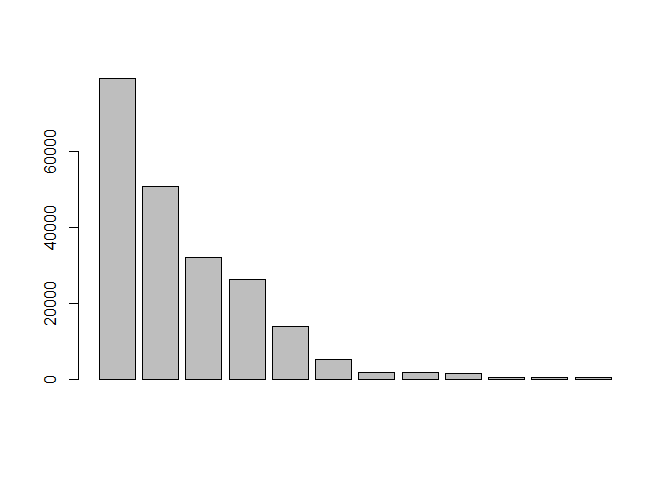
\includegraphics{class05_files/figure-latex/unnamed-chunk-2-1.pdf}

\begin{Shaded}
\begin{Highlighting}[]
\KeywordTok{par}\NormalTok{(}\DataTypeTok{mar=}\KeywordTok{c}\NormalTok{(}\DecValTok{5}\NormalTok{,}\DecValTok{11}\NormalTok{,}\DecValTok{4}\NormalTok{,}\DecValTok{6}\NormalTok{))  }\CommentTok{# changes margins for subsequent plots}
\KeywordTok{barplot}\NormalTok{(features}\OperatorTok{$}\NormalTok{Count, }\DataTypeTok{horiz=}\OtherTok{TRUE}\NormalTok{, }\DataTypeTok{ylab=}\StringTok{""}\NormalTok{, }\DataTypeTok{names.arg=}\NormalTok{features}\OperatorTok{$}\NormalTok{Feature, }\DataTypeTok{main=}\StringTok{"Number of Features in the Mouse GRCm38 Genome"}\NormalTok{, }\DataTypeTok{las=}\DecValTok{1}\NormalTok{)}
\end{Highlighting}
\end{Shaded}

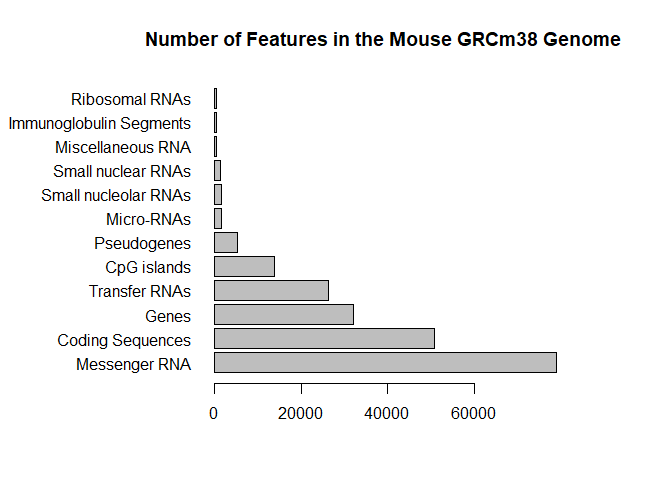
\includegraphics{class05_files/figure-latex/unnamed-chunk-2-2.pdf}

\begin{Shaded}
\begin{Highlighting}[]
\KeywordTok{par}\NormalTok{(}\DataTypeTok{mar=}\KeywordTok{c}\NormalTok{(}\FloatTok{5.1}\NormalTok{,}\FloatTok{4.1}\NormalTok{,}\FloatTok{4.1}\NormalTok{,}\FloatTok{2.1}\NormalTok{))  }\CommentTok{# reset par() for the next plot}
\end{Highlighting}
\end{Shaded}

\textbf{Section 2C}: \emph{HISTOGRAMS}

\begin{Shaded}
\begin{Highlighting}[]
\KeywordTok{hist}\NormalTok{(}\KeywordTok{c}\NormalTok{(}\KeywordTok{rnorm}\NormalTok{(}\DecValTok{10000}\NormalTok{),}\KeywordTok{rnorm}\NormalTok{(}\DecValTok{10000}\NormalTok{)}\OperatorTok{+}\DecValTok{4}\NormalTok{),}\DataTypeTok{breaks=}\DecValTok{50}\NormalTok{, }\DataTypeTok{main=}\StringTok{"sample histogram"}\NormalTok{, }\DataTypeTok{ylab=}\StringTok{""}\NormalTok{, }\DataTypeTok{xlab=}\StringTok{""}\NormalTok{)}
\end{Highlighting}
\end{Shaded}

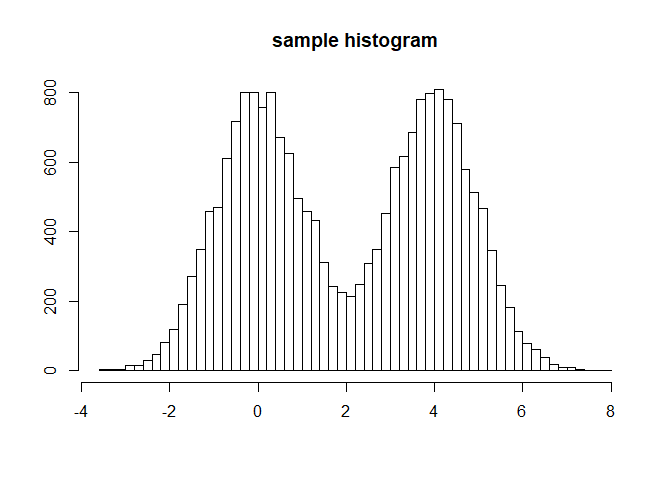
\includegraphics{class05_files/figure-latex/unnamed-chunk-3-1.pdf}

\textbf{Section 3A}: \emph{PROVIDING COLOR VECTORS}

\begin{Shaded}
\begin{Highlighting}[]
\NormalTok{D<-}\KeywordTok{read.delim}\NormalTok{(}\StringTok{"bimm143_05_rstats/male_female_counts.txt"}\NormalTok{)}
   \CommentTok{# shorthand version of read.table() that has defaults header=TRUE and sep="\textbackslash{}t"}
\NormalTok{bar_color<-}\KeywordTok{rainbow}\NormalTok{(}\KeywordTok{nrow}\NormalTok{(D))}
\KeywordTok{barplot}\NormalTok{(D}\OperatorTok{$}\NormalTok{Count, }\DataTypeTok{col=}\NormalTok{bar_color, }\DataTypeTok{ylab=}\StringTok{"Counts"}\NormalTok{, }\DataTypeTok{names.arg=}\NormalTok{D}\OperatorTok{$}\NormalTok{Sample, }\DataTypeTok{las=}\DecValTok{3}\NormalTok{)  }\CommentTok{# rainbow plot... just for kicks}
\end{Highlighting}
\end{Shaded}

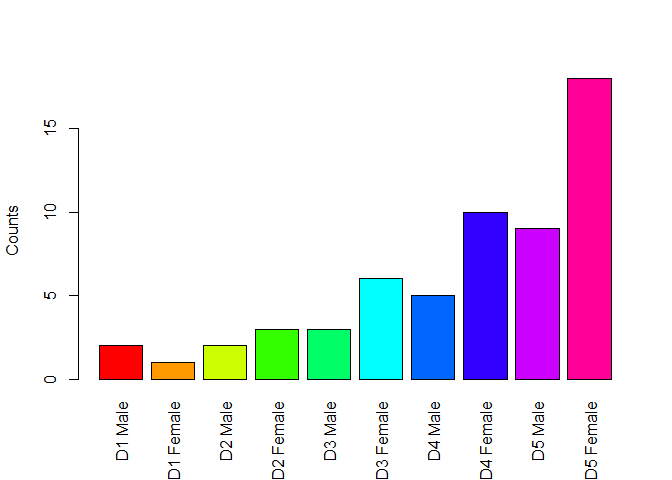
\includegraphics{class05_files/figure-latex/unnamed-chunk-4-1.pdf}

\begin{Shaded}
\begin{Highlighting}[]
\KeywordTok{barplot}\NormalTok{(D}\OperatorTok{$}\NormalTok{Count, }\DataTypeTok{col=}\KeywordTok{c}\NormalTok{(}\StringTok{"cyan"}\NormalTok{,}\StringTok{"magenta"}\NormalTok{), }\DataTypeTok{ylab=}\StringTok{"Counts"}\NormalTok{, }\DataTypeTok{names.arg=}\NormalTok{D}\OperatorTok{$}\NormalTok{Sample, }\DataTypeTok{las=}\DecValTok{3}\NormalTok{)}
\end{Highlighting}
\end{Shaded}

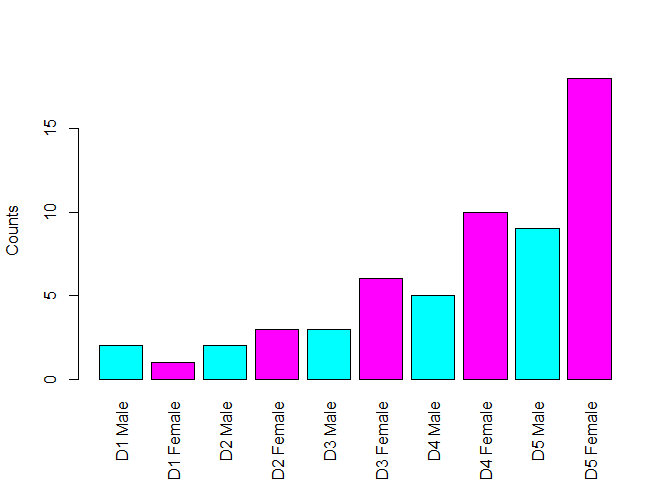
\includegraphics{class05_files/figure-latex/unnamed-chunk-4-2.pdf}

\begin{Shaded}
\begin{Highlighting}[]
\CommentTok{# Need more color schemes? Install Colorspace!}
\CommentTok{# install.packages("colorspace")}
\end{Highlighting}
\end{Shaded}

\textbf{Section 3B}: \emph{COLORING BY VALUE}

\begin{Shaded}
\begin{Highlighting}[]
\NormalTok{genes<-}\KeywordTok{read.delim}\NormalTok{(}\StringTok{"bimm143_05_rstats/up_down_expression.txt"}\NormalTok{)}
\KeywordTok{table}\NormalTok{(genes}\OperatorTok{$}\NormalTok{State)  }\CommentTok{# down: 72, unchanging: 4997, up: 127}
\end{Highlighting}
\end{Shaded}

\begin{verbatim}
## 
##       down unchanging         up 
##         72       4997        127
\end{verbatim}

\begin{Shaded}
\begin{Highlighting}[]
\NormalTok{defaultpalette<-}\KeywordTok{palette}\NormalTok{()          }\CommentTok{# save default palette}
\KeywordTok{palette}\NormalTok{(}\KeywordTok{c}\NormalTok{(}\StringTok{"blue"}\NormalTok{, }\StringTok{"gray"}\NormalTok{, }\StringTok{"red"}\NormalTok{))  }\CommentTok{# change palette colors for the graph}
\KeywordTok{plot}\NormalTok{(genes}\OperatorTok{$}\NormalTok{Condition1, genes}\OperatorTok{$}\NormalTok{Condition2, }\DataTypeTok{col=}\NormalTok{genes}\OperatorTok{$}\NormalTok{State, }\DataTypeTok{xlab=}\StringTok{"Expression Condition 1"}\NormalTok{, }\DataTypeTok{ylab=}\StringTok{"Expression Condition 2"}\NormalTok{)}
\end{Highlighting}
\end{Shaded}

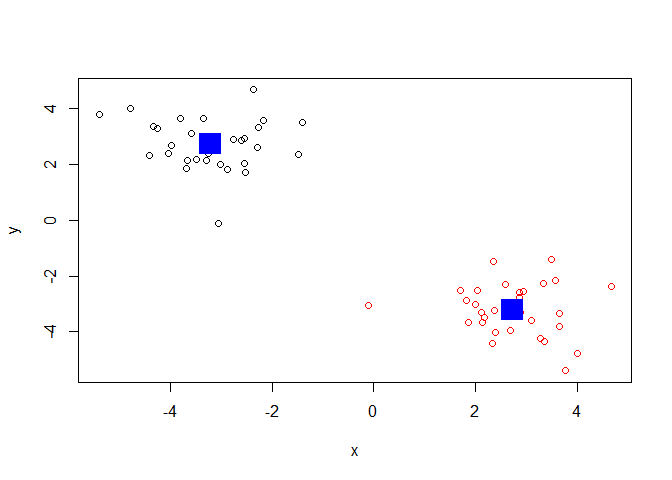
\includegraphics{class05_files/figure-latex/unnamed-chunk-5-1.pdf}

\begin{Shaded}
\begin{Highlighting}[]
\KeywordTok{palette}\NormalTok{(defaultpalette)            }\CommentTok{# reset palette colors}
\end{Highlighting}
\end{Shaded}

\textbf{Section 3C}: \emph{DYNAMIC USE OF COLOR}

\begin{Shaded}
\begin{Highlighting}[]
\NormalTok{methylation<-}\KeywordTok{read.delim}\NormalTok{(}\StringTok{"bimm143_05_rstats/expression_methylation.txt"}\NormalTok{)}
\KeywordTok{nrow}\NormalTok{(methylation)  }\CommentTok{# 9241}
\end{Highlighting}
\end{Shaded}

\begin{verbatim}
## [1] 9241
\end{verbatim}

\begin{Shaded}
\begin{Highlighting}[]
\KeywordTok{plot}\NormalTok{(methylation}\OperatorTok{$}\NormalTok{gene.meth, methylation}\OperatorTok{$}\NormalTok{expression)  }\CommentTok{# difficult to interpret}
\end{Highlighting}
\end{Shaded}

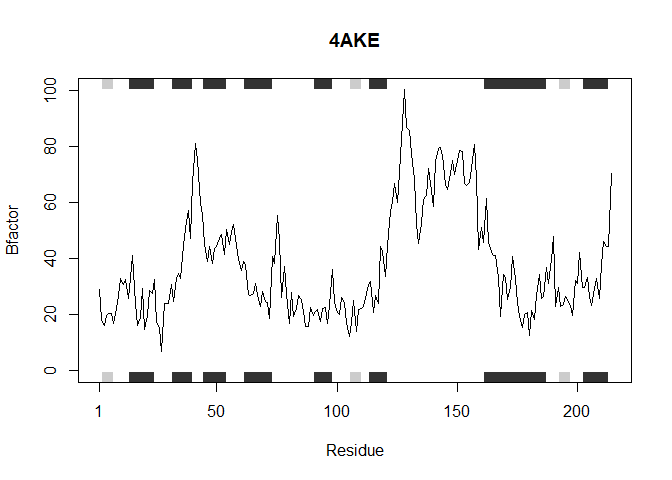
\includegraphics{class05_files/figure-latex/unnamed-chunk-6-1.pdf}

\begin{Shaded}
\begin{Highlighting}[]
\NormalTok{heatmap_blue<-}\KeywordTok{densCols}\NormalTok{(methylation}\OperatorTok{$}\NormalTok{gene.meth, methylation}\OperatorTok{$}\NormalTok{expression)}
\KeywordTok{plot}\NormalTok{(methylation}\OperatorTok{$}\NormalTok{gene.meth, methylation}\OperatorTok{$}\NormalTok{expression, }\DataTypeTok{col=}\NormalTok{heatmap_blue)  }\CommentTok{# so many zeros!}
\end{Highlighting}
\end{Shaded}

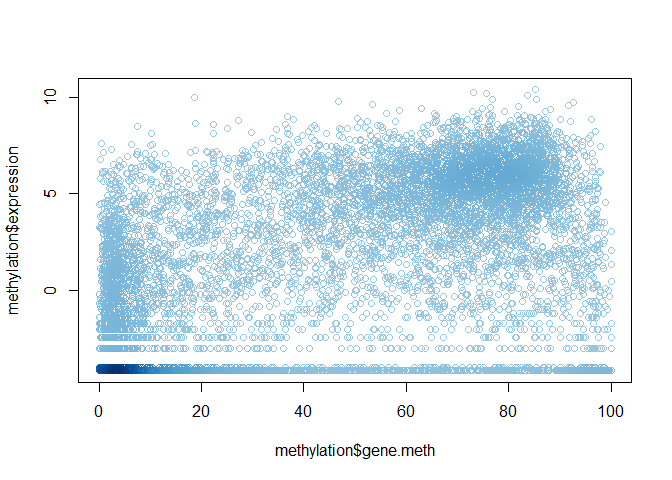
\includegraphics{class05_files/figure-latex/unnamed-chunk-6-2.pdf}

\begin{Shaded}
\begin{Highlighting}[]
\NormalTok{posexpr<-methylation}\OperatorTok{$}\NormalTok{expression}\OperatorTok{>}\DecValTok{0}
\NormalTok{heatmap_blue2<-}\KeywordTok{densCols}\NormalTok{(methylation}\OperatorTok{$}\NormalTok{gene.meth[posexpr], methylation}\OperatorTok{$}\NormalTok{expression[posexpr])}
\KeywordTok{plot}\NormalTok{(methylation}\OperatorTok{$}\NormalTok{gene.meth[posexpr], methylation}\OperatorTok{$}\NormalTok{expression[posexpr], }\DataTypeTok{col=}\NormalTok{heatmap_blue2)  }\CommentTok{# nice!}
\end{Highlighting}
\end{Shaded}

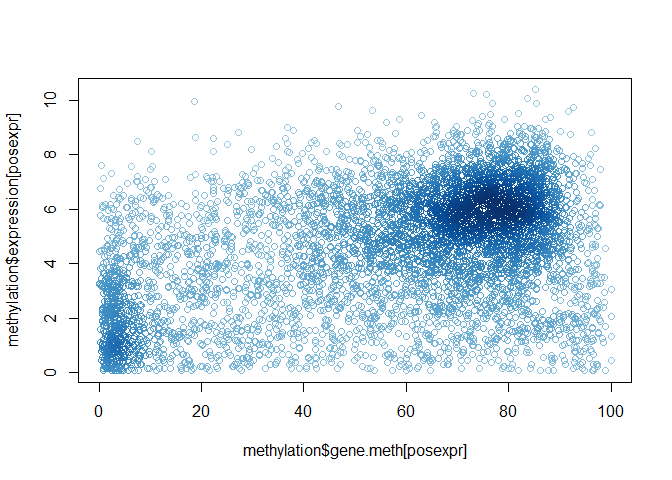
\includegraphics{class05_files/figure-latex/unnamed-chunk-6-3.pdf}

\begin{Shaded}
\begin{Highlighting}[]
\NormalTok{heatmap_color<-}\KeywordTok{densCols}\NormalTok{(methylation}\OperatorTok{$}\NormalTok{gene.meth[posexpr], methylation}\OperatorTok{$}\NormalTok{expression[posexpr], }\DataTypeTok{colramp=}\KeywordTok{colorRampPalette}\NormalTok{(}\KeywordTok{c}\NormalTok{(}\StringTok{"blue"}\NormalTok{, }\StringTok{"green"}\NormalTok{, }\StringTok{"yellow"}\NormalTok{, }\StringTok{"red"}\NormalTok{)))}
\KeywordTok{plot}\NormalTok{(methylation}\OperatorTok{$}\NormalTok{gene.meth[posexpr], methylation}\OperatorTok{$}\NormalTok{expression[posexpr], }\DataTypeTok{col=}\NormalTok{heatmap_color)  }\CommentTok{# colorful!}
\end{Highlighting}
\end{Shaded}

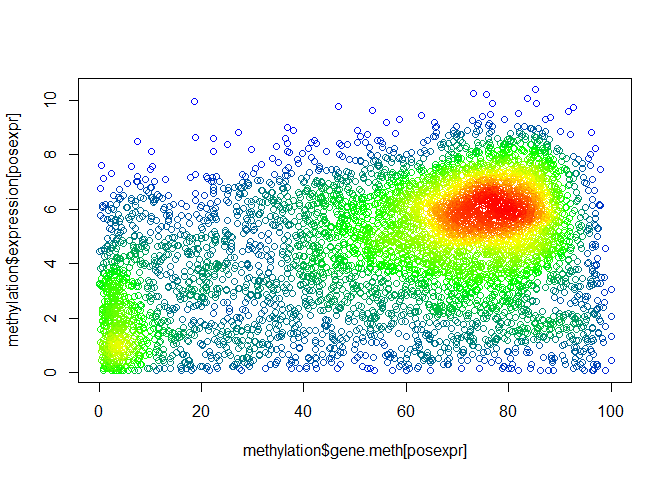
\includegraphics{class05_files/figure-latex/unnamed-chunk-6-4.pdf}

\begin{Shaded}
\begin{Highlighting}[]
\KeywordTok{plot}\NormalTok{(methylation}\OperatorTok{$}\NormalTok{gene.meth[posexpr], methylation}\OperatorTok{$}\NormalTok{expression[posexpr], }\DataTypeTok{col=}\NormalTok{heatmap_color, }\DataTypeTok{pch=}\DecValTok{20}\NormalTok{)  }\CommentTok{# filled circles}
\end{Highlighting}
\end{Shaded}

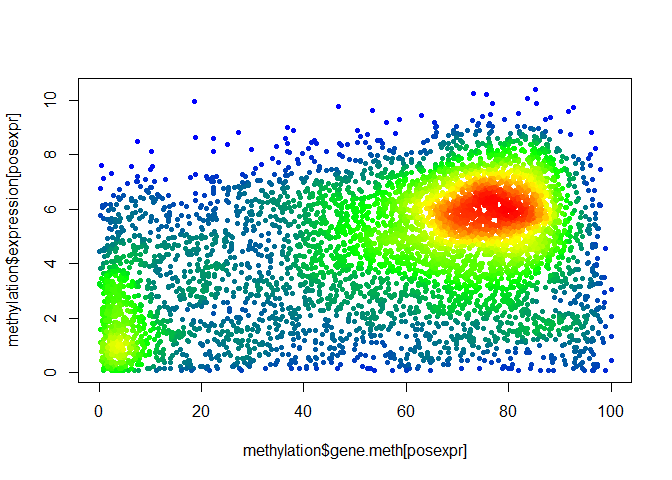
\includegraphics{class05_files/figure-latex/unnamed-chunk-6-5.pdf}

\textbf{Section 4}: \emph{MAPPING COLORS}

\begin{Shaded}
\begin{Highlighting}[]
\CommentTok{# function from color_to_value_map.r}
\NormalTok{map.colors <-}\StringTok{ }\ControlFlowTok{function}\NormalTok{ (value,high.low,palette) \{}
\NormalTok{  proportion <-}\StringTok{ }\NormalTok{((value}\OperatorTok{-}\NormalTok{high.low[}\DecValTok{1}\NormalTok{])}\OperatorTok{/}\NormalTok{(high.low[}\DecValTok{2}\NormalTok{]}\OperatorTok{-}\NormalTok{high.low[}\DecValTok{1}\NormalTok{]))}
\NormalTok{  index <-}\StringTok{ }\KeywordTok{round}\NormalTok{ ((}\KeywordTok{length}\NormalTok{(palette)}\OperatorTok{-}\DecValTok{1}\NormalTok{)}\OperatorTok{*}\NormalTok{proportion)}\OperatorTok{+}\DecValTok{1}
  \KeywordTok{return}\NormalTok{ (palette[index])}
\NormalTok{\}}
\CommentTok{# plot promoter vs gene from methylation dataset}
\KeywordTok{plot}\NormalTok{(methylation}\OperatorTok{$}\NormalTok{promoter.meth, methylation}\OperatorTok{$}\NormalTok{gene.meth, }\DataTypeTok{xlab=}\StringTok{"Promoter Methylation"}\NormalTok{, }\DataTypeTok{ylab=}\StringTok{"Gene Methylation"}\NormalTok{)}
\end{Highlighting}
\end{Shaded}

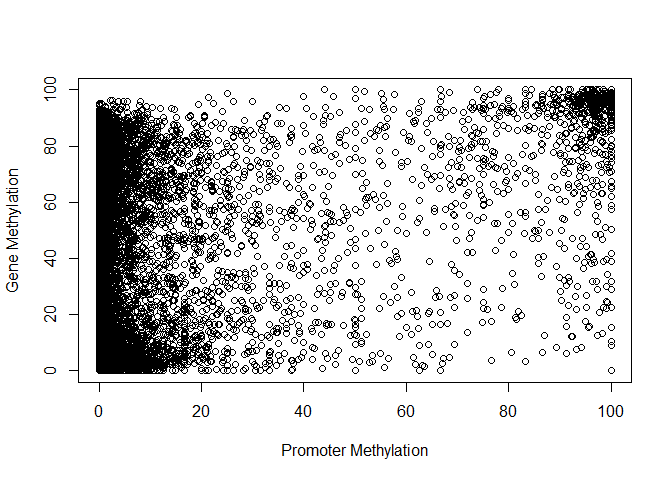
\includegraphics{class05_files/figure-latex/unnamed-chunk-7-1.pdf}

\begin{Shaded}
\begin{Highlighting}[]
\NormalTok{shadesofgred<-}\KeywordTok{colorRampPalette}\NormalTok{(}\KeywordTok{c}\NormalTok{(}\StringTok{"gray"}\NormalTok{,}\StringTok{"red"}\NormalTok{))}
\NormalTok{shadesofgred100<-}\KeywordTok{colorRampPalette}\NormalTok{(}\KeywordTok{c}\NormalTok{(}\StringTok{"gray"}\NormalTok{,}\StringTok{"red"}\NormalTok{))(}\DecValTok{100}\NormalTok{)}
\NormalTok{gred<-}\KeywordTok{map.colors}\NormalTok{(methylation}\OperatorTok{$}\NormalTok{expression,}\KeywordTok{c}\NormalTok{(}\KeywordTok{max}\NormalTok{(methylation}\OperatorTok{$}\NormalTok{expression),}\KeywordTok{min}\NormalTok{(methylation}\OperatorTok{$}\NormalTok{expression)),shadesofgred100)}
\KeywordTok{plot}\NormalTok{(methylation}\OperatorTok{$}\NormalTok{promoter.meth, methylation}\OperatorTok{$}\NormalTok{gene.meth, }\DataTypeTok{xlab=}\StringTok{"Promoter Methylation"}\NormalTok{, }\DataTypeTok{ylab=}\StringTok{"Gene Methylation"}\NormalTok{, }\DataTypeTok{col=}\NormalTok{gred)  }\CommentTok{# red and gray points}
\end{Highlighting}
\end{Shaded}

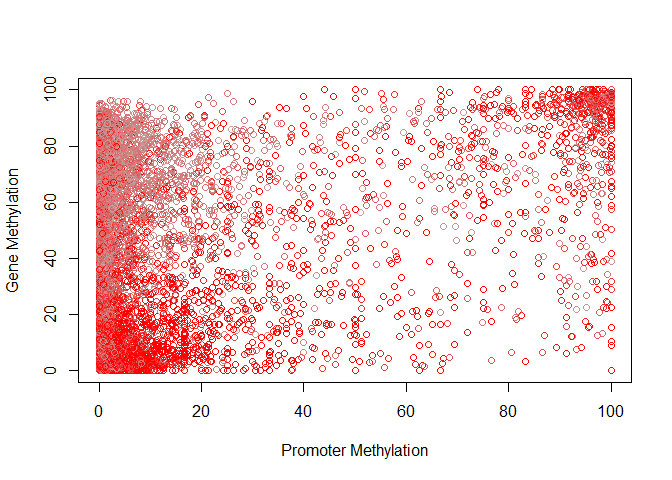
\includegraphics{class05_files/figure-latex/unnamed-chunk-7-2.pdf}

\begin{Shaded}
\begin{Highlighting}[]
\KeywordTok{plot}\NormalTok{(methylation}\OperatorTok{$}\NormalTok{promoter.meth, methylation}\OperatorTok{$}\NormalTok{gene.meth, }\DataTypeTok{xlab=}\StringTok{"Promoter Methylation"}\NormalTok{, }\DataTypeTok{ylab=}\StringTok{"Gene Methylation"}\NormalTok{, }\DataTypeTok{col=}\KeywordTok{map.colors}\NormalTok{(methylation}\OperatorTok{$}\NormalTok{expression,}\KeywordTok{c}\NormalTok{(}\KeywordTok{max}\NormalTok{(methylation}\OperatorTok{$}\NormalTok{expression),}\KeywordTok{min}\NormalTok{(methylation}\OperatorTok{$}\NormalTok{expression)),}\KeywordTok{colorRampPalette}\NormalTok{(}\KeywordTok{c}\NormalTok{(}\StringTok{"blue"}\NormalTok{,}\StringTok{"red"}\NormalTok{))(}\DecValTok{100}\NormalTok{)))  }\CommentTok{# red and blue points}
\end{Highlighting}
\end{Shaded}

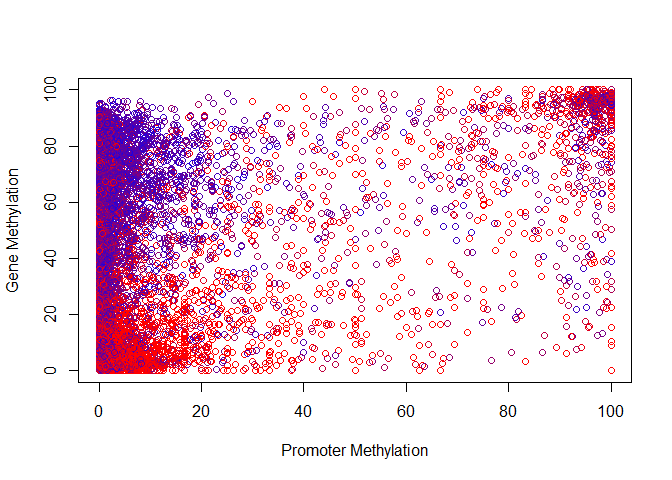
\includegraphics{class05_files/figure-latex/unnamed-chunk-7-3.pdf}


\end{document}
